\chapter{The application}\label{ch:app}

\section{Interface}
The interface follows two rules: the customer should always be able to read what the system understood, and nothing should look different from everything else. Type is Inter for the interface and Bodoni Moda for headlines, on white. Every control is a rounded pill or card from one set of shapes; the views are switched by a segmented control; editing a detail opens a sheet that slides up over the page. The home page (Figure~\ref{fig:home}) says what the service does and starts a design. Its centrepiece is a sphere rendered live on the GPU by a fragment shader (noise-displaced surface, specular highlight, thin-film iridescence at grazing angles) that breathes when idle and ripples with the voice level while the customer speaks; without WebGL it falls back to a still image of the same look.

\begin{figure}[tbp]
\centering
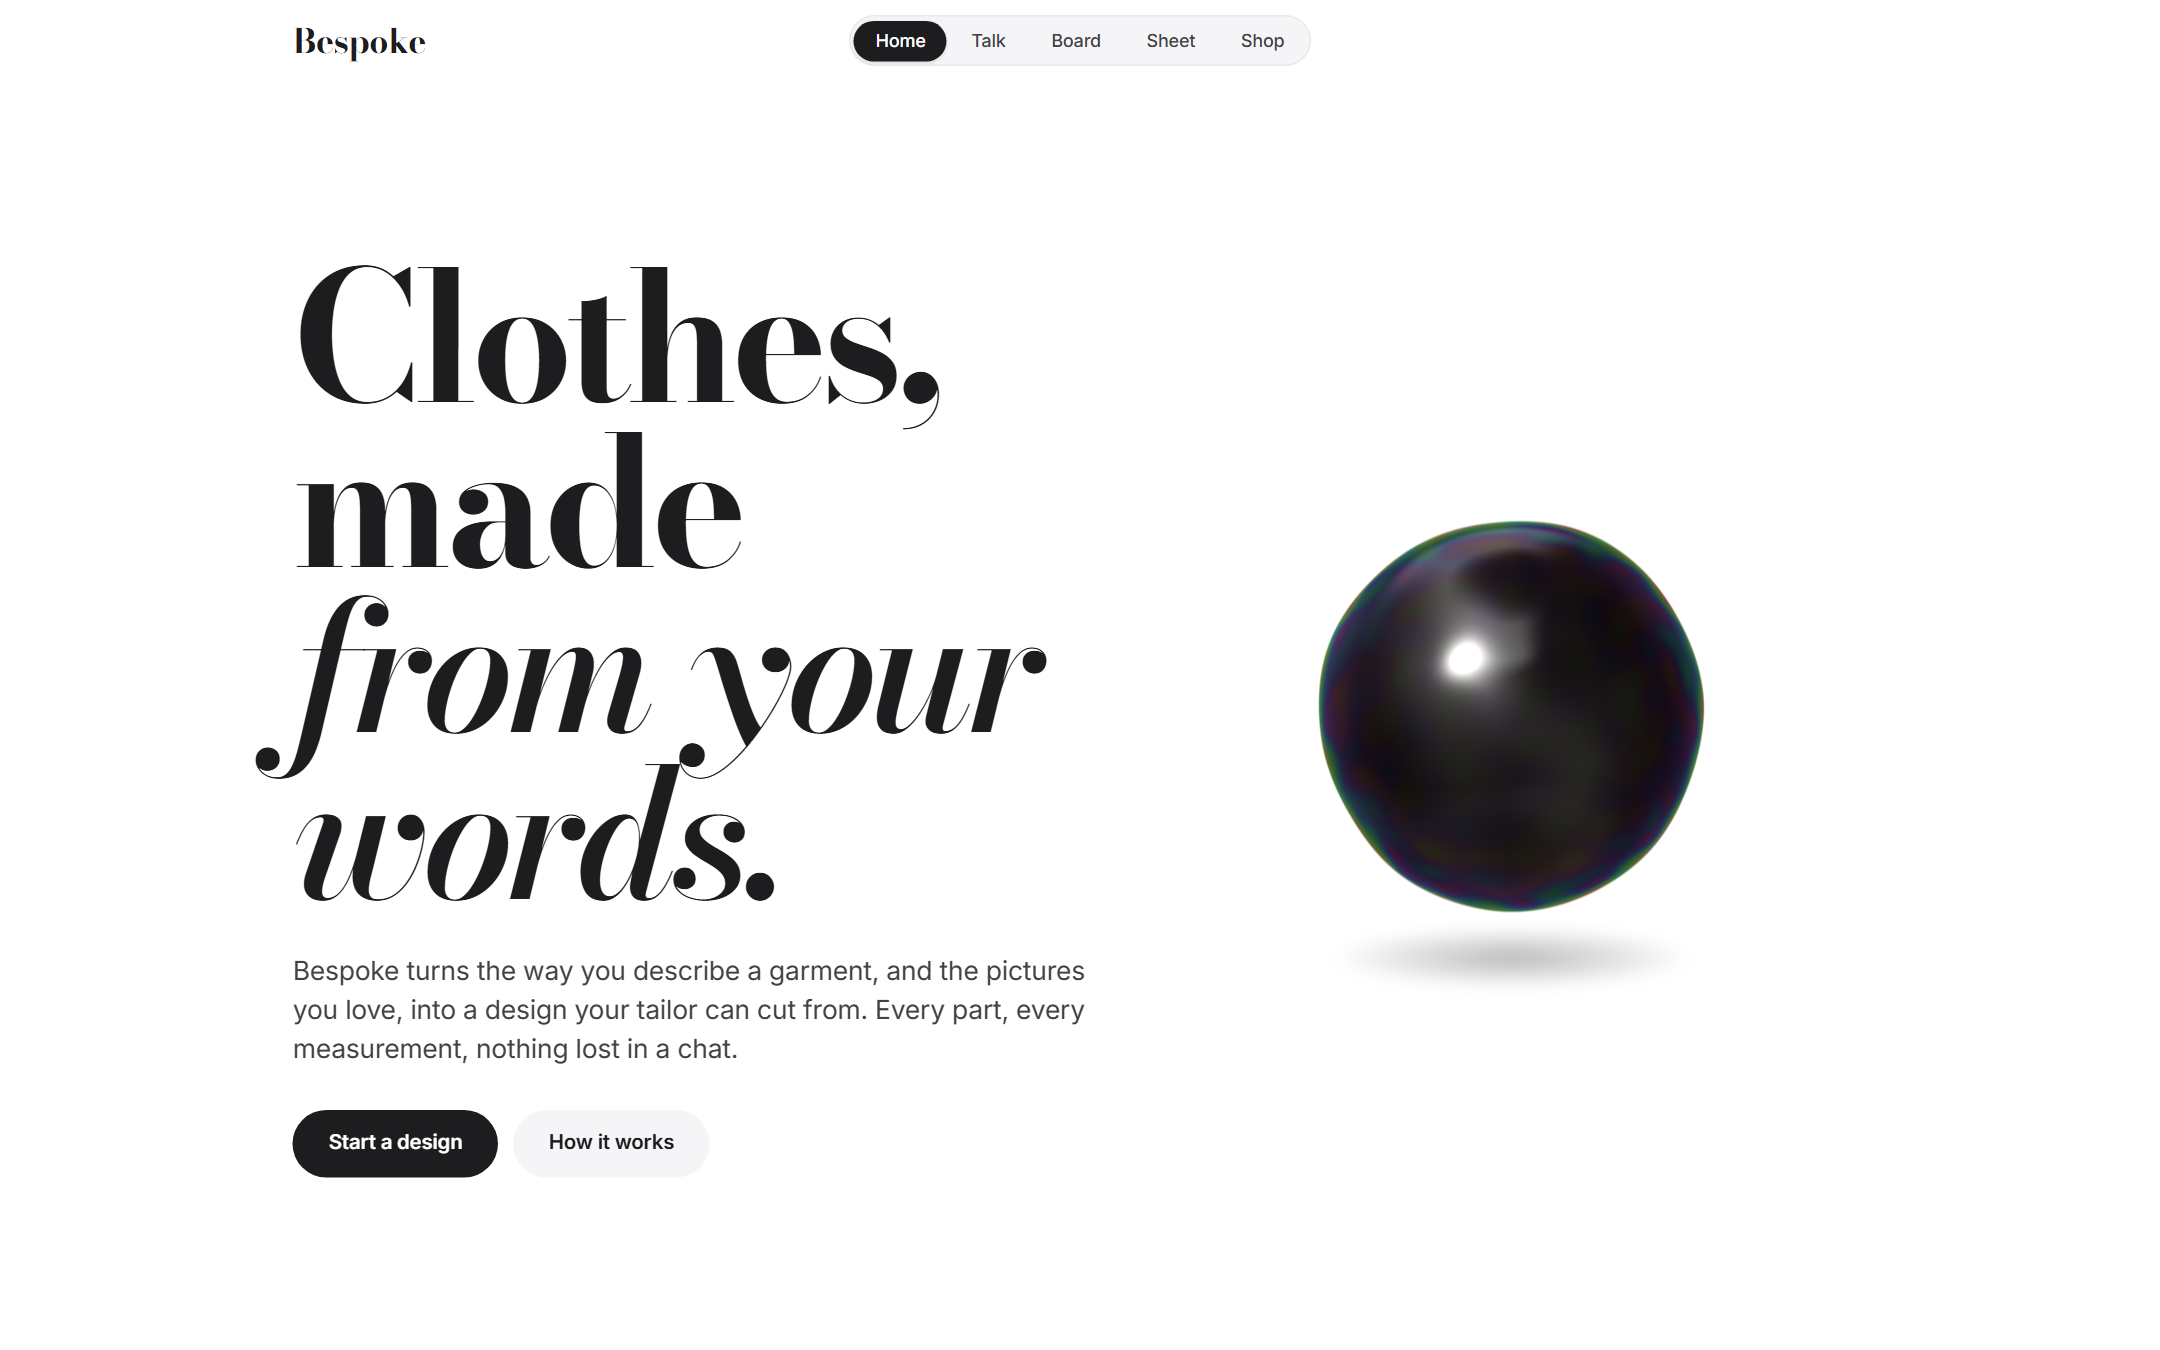
\includegraphics[width=\linewidth]{img/home.png}
\caption{The home page at desktop width.}
\label{fig:home}
\end{figure}

\section{The conversation}
The conversation view (Figure~\ref{fig:talk}) answers in one sentence, shows the request with the understood words underlined, and lists the design on an order card: each row a slot, its value, and where it came from. Any row can be changed by tapping it, which opens a picker; for colour the picker is a palette with a shade maker that records the exact shade as a note for the tailor. At most two questions are asked per turn. Every step can be taken back: before each message, answer, edit or board reading the design and the conversation are saved, and a Back button under the latest reply restores the previous state exactly, up to thirty steps. When the design is complete, the tailor sheet and the shopping links appear in the conversation itself, so the customer is not sent elsewhere to finish.

\begin{figure}[tbp]
\centering
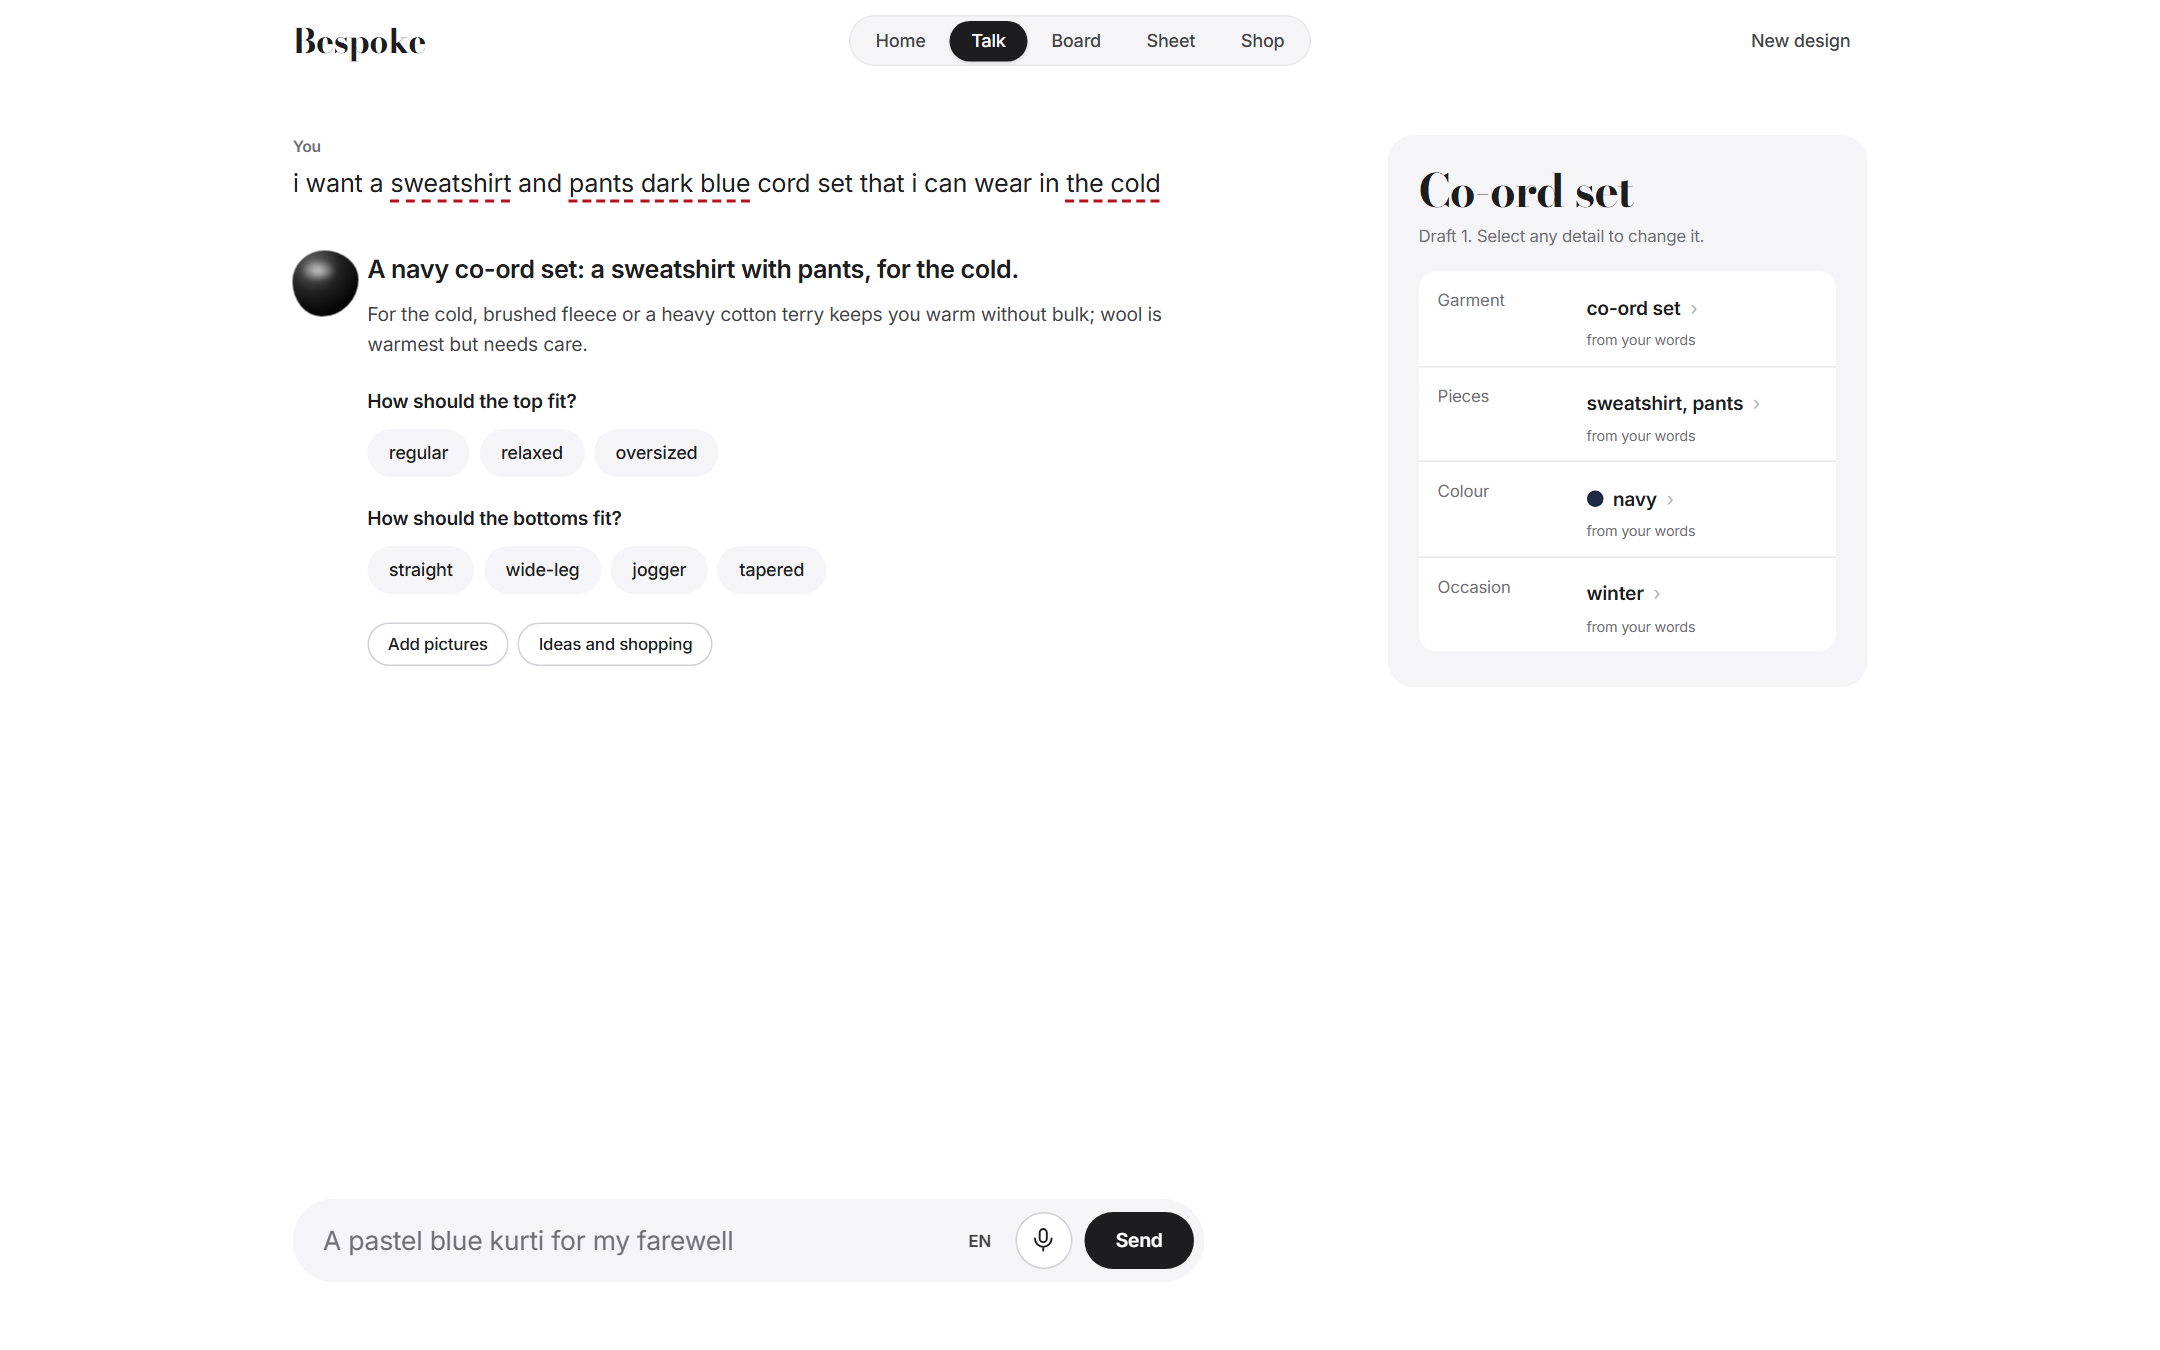
\includegraphics[width=\linewidth]{img/talk.png}
\caption{The request that the first version misread, now a navy co-ord set for winter. The questions are about fit and warm fabrics; there is no neckline question for a sweatshirt.}
\label{fig:talk}
\end{figure}

\section{The moodboard}
The board is an embedded Excalidraw canvas \cite{excalidraw}, used under its MIT licence, with its own menu and the licence notice kept in the site's open-source notices. Customers drop or paste pictures, write notes, draw arrows from a note to the picture it describes and circle the part they like. Reading the board numbers the pictures and scores each one with CLIP zero-shot \cite{radford2021clip}, on the device. Only garment, colour and print are read from a whole picture, because zero-shot scores for necklines and sleeves on unconstrained photos proved unreliable; those are read only from circled regions. A value from pictures is used only if its probability is at least 0.55 and leads the next by 0.2, and its confidence is capped at 0.6, so it can fill a gap but never overrule what the customer wrote.

\section{The tailor sheet}
The sheet (Figure~\ref{fig:sheet}) lists every instruction by part with its source, so the tailor can tell the customer's words from a default. It switches wholly to Hindi, including part names, values, labels and the finished measurements, which are the customer's body measurements plus the ease the fit implies. Drawings of the chosen neckline, sleeves, shape, length and fabric are printed beside the instructions once the picture library is published. The sheet prints to A4 or saves as PDF.

\begin{figure}[tbp]
\centering
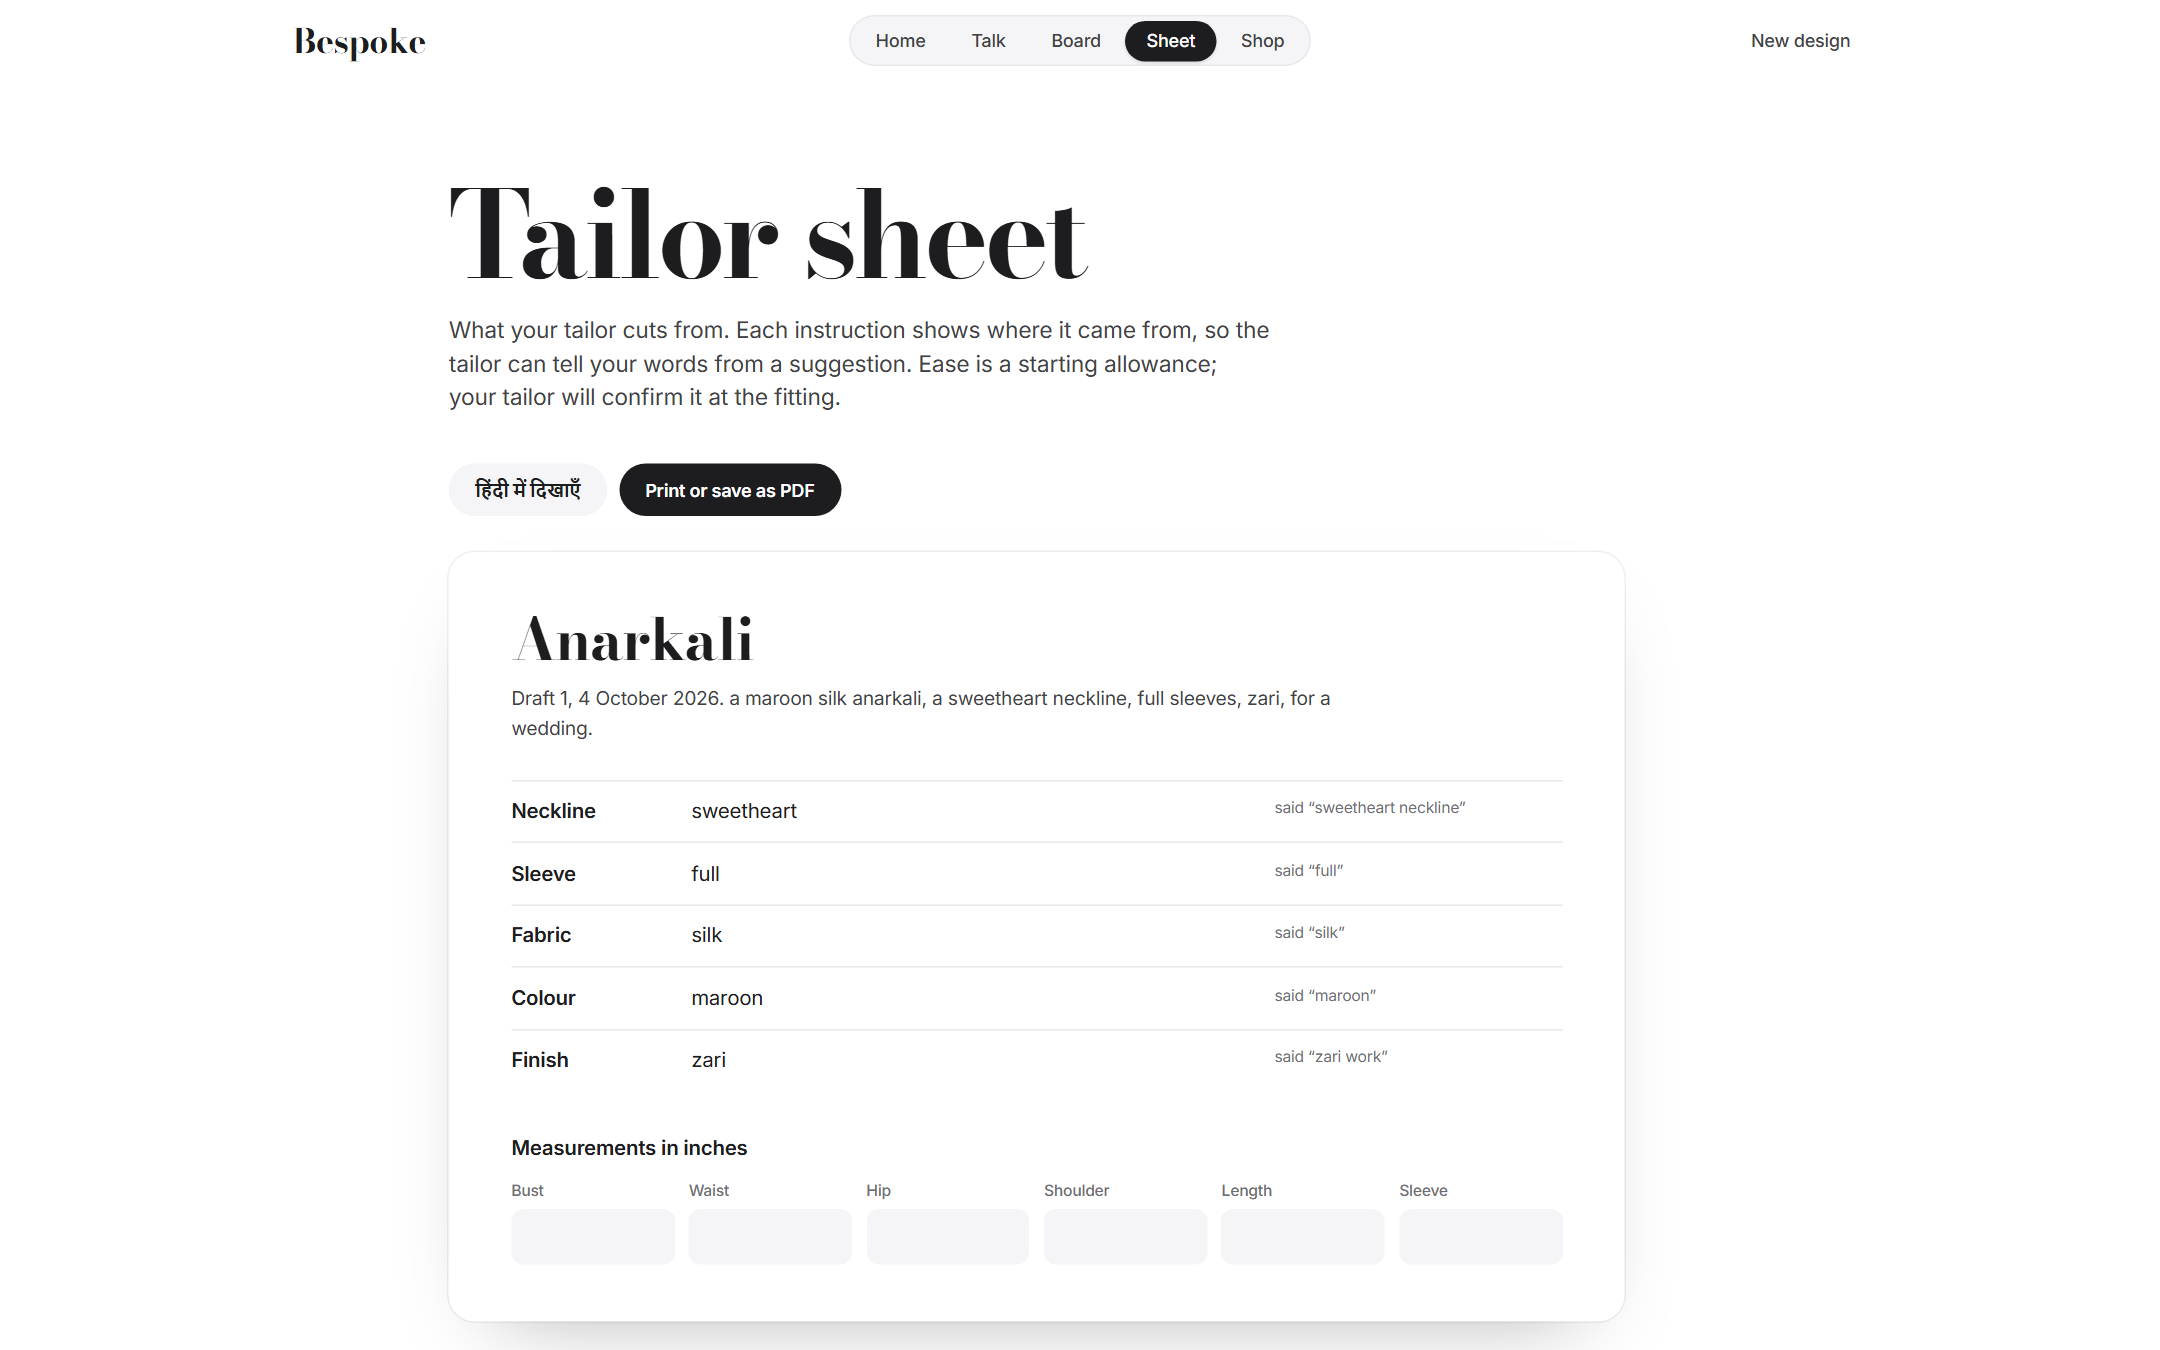
\includegraphics[width=0.49\linewidth]{img/sheet.png}\hfill
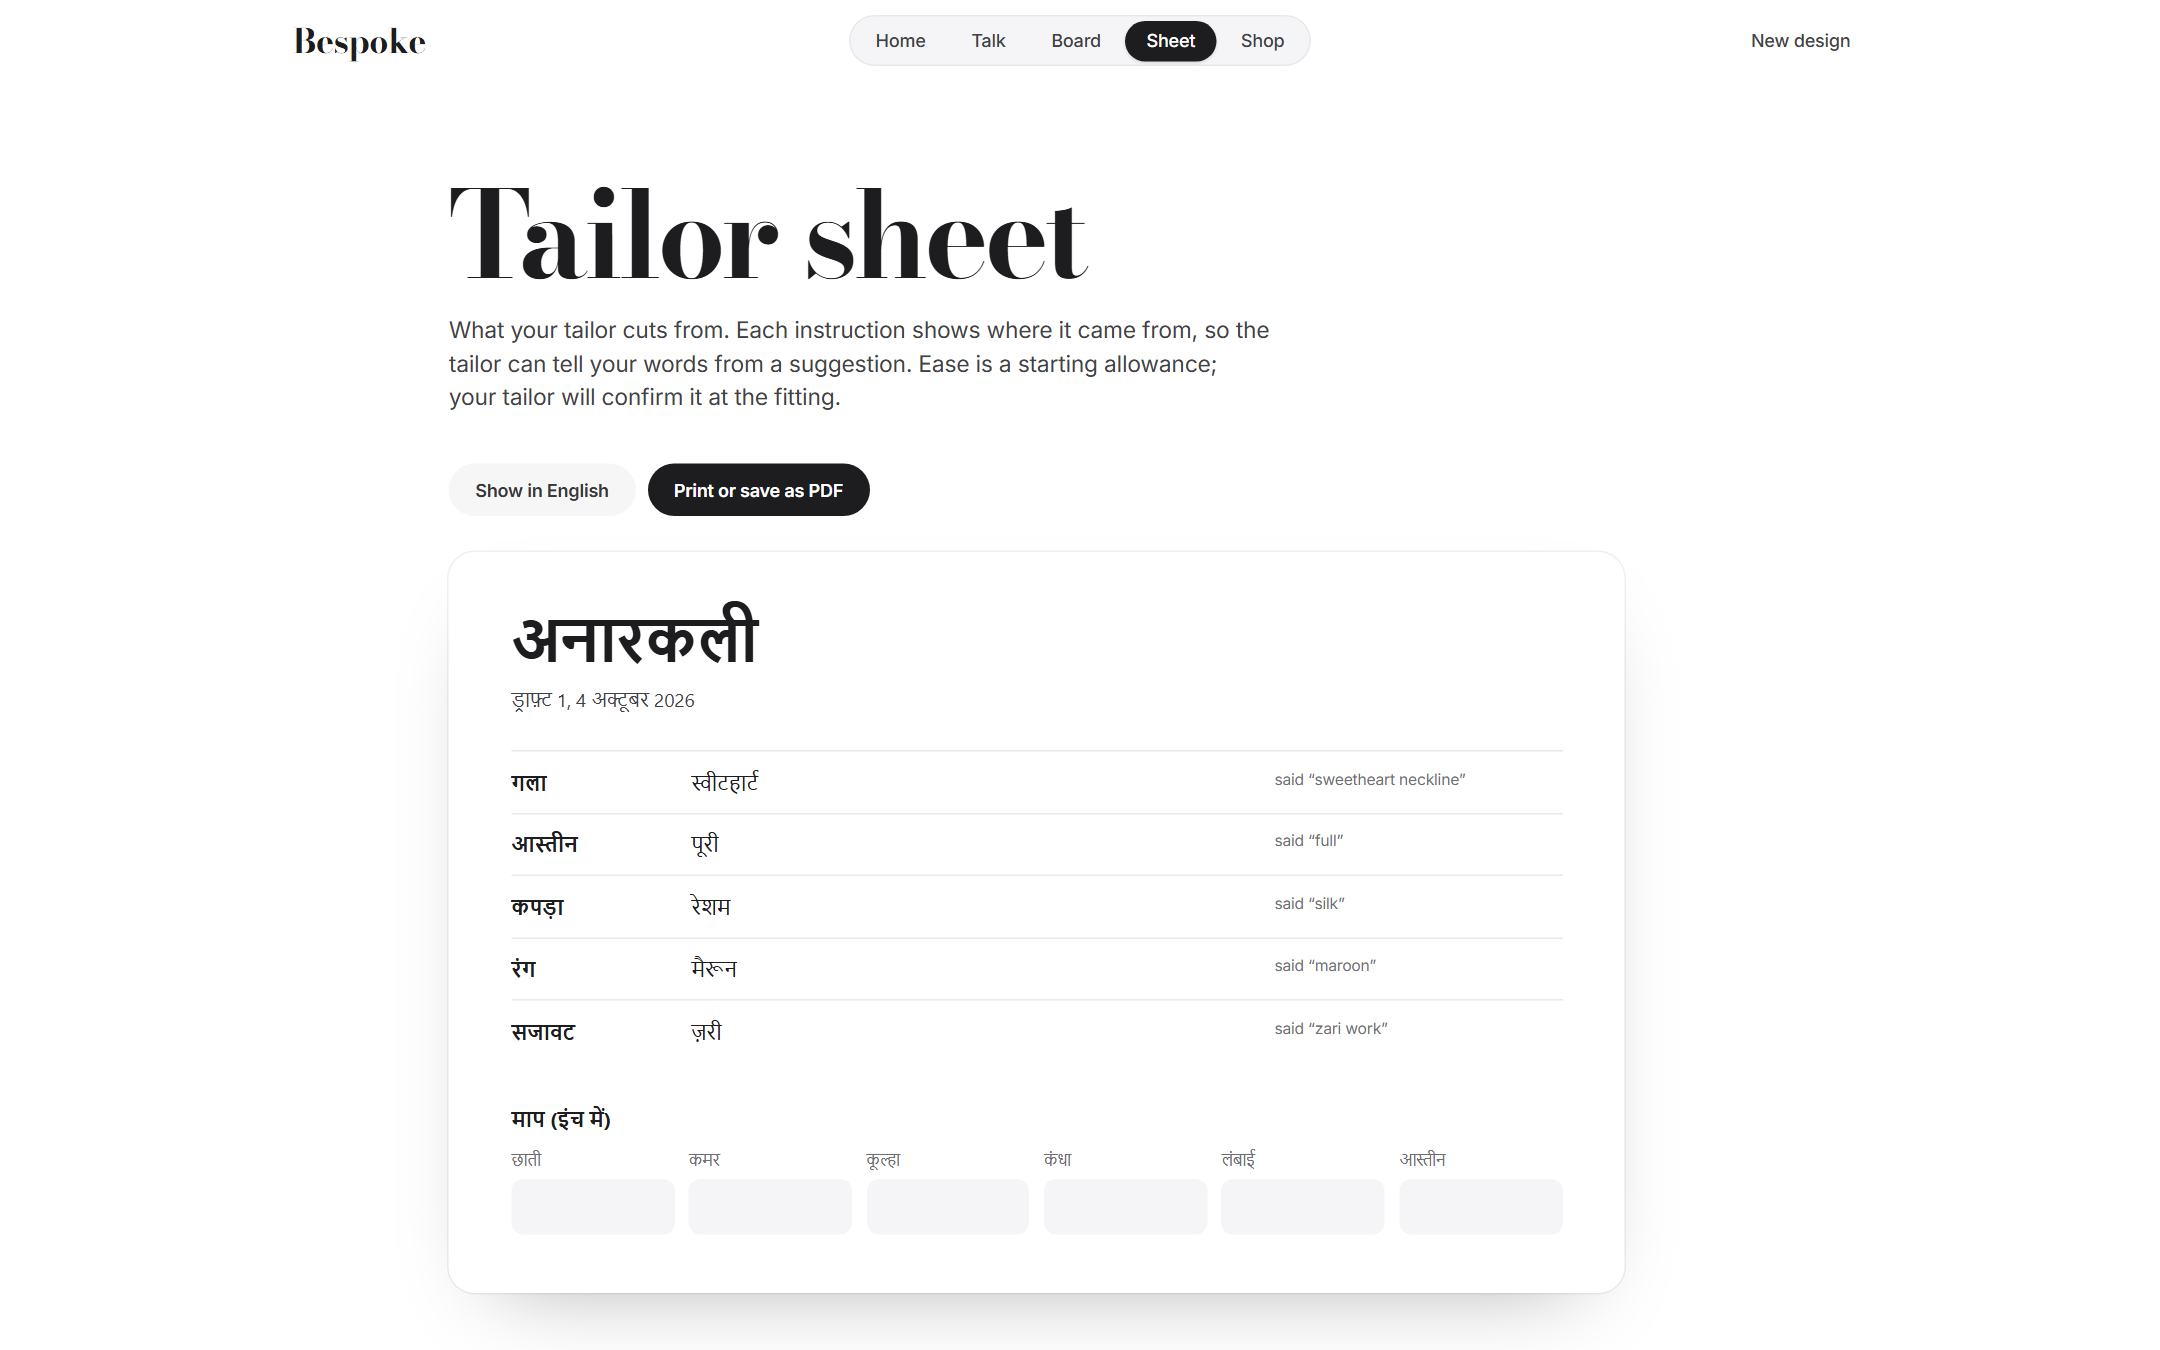
\includegraphics[width=0.49\linewidth]{img/sheet-hi.png}
\caption{The same tailor sheet in English and in Hindi.}
\label{fig:sheet}
\end{figure}

\section{Shopping and ideas}
The shop view writes one search from the design and opens it on Myntra, Ajio, Amazon, Flipkart and Nykaa Fashion, with Pinterest searches for ideas, fabric by the metre and tailors nearby on a map. Searches for garments worn by everyone are prefixed with the wearer, which the binder infers from the request and the customer can switch between women, men and anyone. Pinterest content is linked, not copied: its terms forbid storing pins or training on them.

\section{Deployment}
The site is a static export of a Next.js application, deployed on Vercel from the public repository \code{riteshroshann/onestyle}, with one serverless function for the optional model layer. The model key is held only in the host's environment. With no key the site is complete; the function answers 501 and the page uses the engine alone. The site works on phones, where the navigation stacks under the brand and every control is at least 32 pixels tall (Figure~\ref{fig:phone}).

\begin{figure}[tbp]
\centering
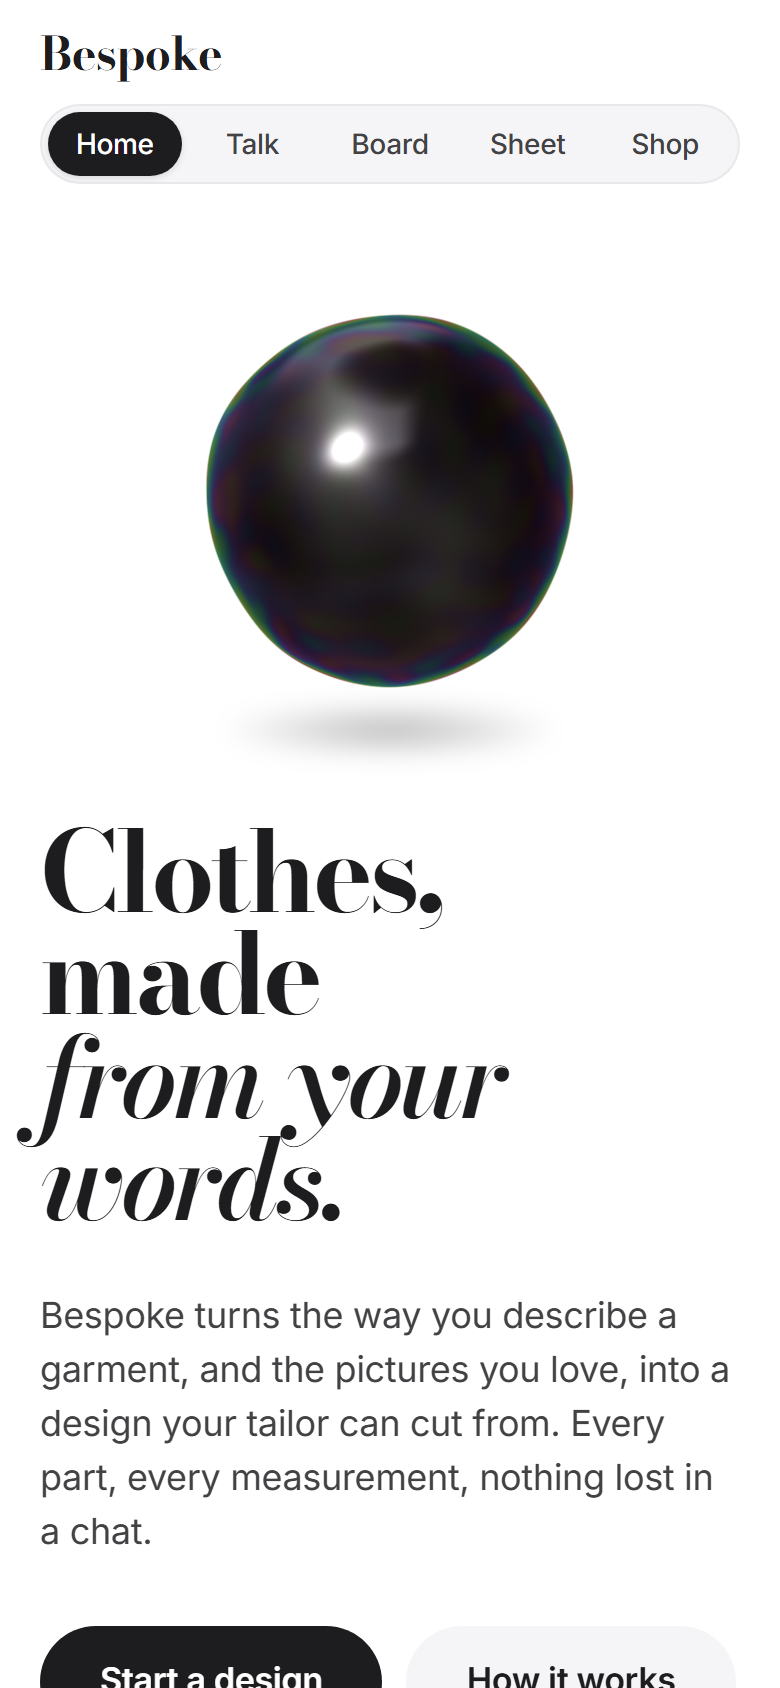
\includegraphics[width=0.3\linewidth]{img/phone.png}
\caption{The home page on a 390-pixel phone.}
\label{fig:phone}
\end{figure}
